\section{Resultados}
\subsection{Poblaciones inferidas desde el exceso observado}
La condición inversa reconstruyó poblaciones separadas compatibles con $Y_{\Delta B}^{\rm ref}=8.6932\times10^{-11}$, bajo las condiciones térmicas declaradas. Con PDG2025, a 150 MeV se obtuvo $\mu_B/T=1.1647\times10^{-8}$ y
\begin{align}
n_B&\simeq1.7222\times10^{37}\ {\rm cm^{-3}},\\
n_{\bar B}&\simeq1.7222\times10^{37}\ {\rm cm^{-3}},\\
\Delta n_B&=4.0110\times10^{29}\ {\rm cm^{-3}}.
\label{eq:inferredinitial}
\end{align}
Los dos primeros valores coinciden al redondeo mostrado, pero no son iguales: $n_{\bar B}/n_B=0.9999999767$. El total fue $3.4444\times10^{37}$ cm$^{-3}$ y la contabilidad de pares potenciales, $\min(n_B,n_{\bar B})\simeq1.7222\times10^{37}$ cm$^{-3}$. Son cantidades medias por volumen físico del plasma a esa temperatura.

A 40 MeV, el mismo exceso por entropía dio $\mu_B/T=0.1261002$, $n_B=1.9166\times10^{28}$ y $n_{\bar B}=1.4894\times10^{28}$ cm$^{-3}$. La diferencia fue $4.2724\times10^{27}$ cm$^{-3}$ y la razón $n_{\bar B}/n_B=0.777089$. La Tabla~\ref{tab:inversepop} presenta la secuencia completa. El rendimiento total bajó de $7.4653\times10^{-3}$ a $6.9304\times10^{-10}$, una reducción de 7.0323 órdenes de magnitud. Su cociente respecto del exceso neto fue $8.5875\times10^7$ al inicio y 7.9722 al final de la malla (Figura~\ref{fig:inverse}).

\begin{table*}[t]\centering\small
\caption{Reconstrucción inversa propia con PDG2025 y $Y_{\Delta B}=\eta/7.04$ como condición externa. Las densidades son medias por volumen físico; coinciden al redondeo en temperaturas altas, pero conservan un exceso finito. $\alpha=\mu_B/T$ y $Y_\Sigma=n_\Sigma/s_{\rm tot}$. Se usaron entradas centrales, sin errores físicos asignados al HRG.}\label{tab:inversepop}
\setlength{\tabcolsep}{7pt}\renewcommand{\arraystretch}{1.14}
\begin{tabular}{rrrrrr}\toprule
$T$ (MeV) & $\alpha$ & $n_B$ (${\rm cm^{-3}}$) & $n_{\bar B}$ (${\rm cm^{-3}}$) & $Y_\Sigma$ & $n_{\bar B}/n_B$ \\ \midrule
150 & $1.165\times10^{-8}$ & $1.722\times10^{37}$ & $1.722\times10^{37}$ & 0.007465 & 1.000000 \\
140 & $1.779\times10^{-8}$ & $8.354\times10^{36}$ & $8.354\times10^{36}$ & 0.004887 & 1.000000 \\
120 & $5.319\times10^{-8}$ & $1.525\times10^{36}$ & $1.525\times10^{36}$ & 0.001634 & 1.000000 \\
100 & $2.480\times10^{-7}$ & $1.720\times10^{35}$ & $1.720\times10^{35}$ & $3.506\times10^{-4}$ & 1.000000 \\
80 & $2.358\times10^{-6}$ & $8.643\times10^{33}$ & $8.643\times10^{33}$ & $3.687\times10^{-5}$ & 0.999995 \\
60 & $9.060\times10^{-5}$ & $8.860\times10^{31}$ & $8.858\times10^{31}$ & $9.595\times10^{-7}$ & 0.999819 \\
50 & 0.001631 & $2.726\times10^{30}$ & $2.717\times10^{30}$ & $5.331\times10^{-8}$ & 0.996744 \\
40 & 0.1261 & $1.917\times10^{28}$ & $1.489\times10^{28}$ & $6.930\times10^{-10}$ & 0.777089 \\
\bottomrule\end{tabular}\end{table*}

\begin{figure*}[t]
\centering
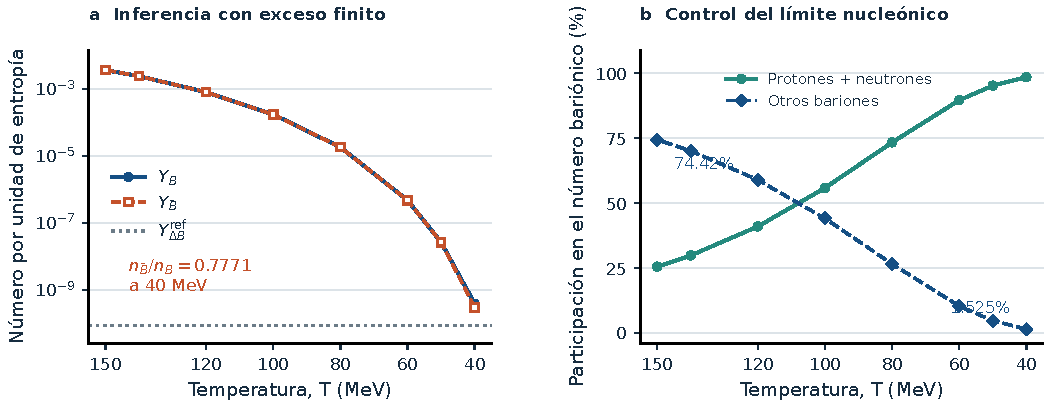
\includegraphics[width=.99\textwidth]{figures/fig05_inverse_es.pdf}
\caption{Resultados propios que responden al objetivo retrospectivo. (a) Rendimientos de bariones y antibariones inferidos con PDG2025 y el exceso publicado como condición de entrada. Las curvas casi coinciden a temperaturas altas; su diferencia aumenta en proporción al total al enfriar. La línea gris es la condición externa conservada. (b) Participación de protones y neutrones, y de los restantes bariones, en el control simétrico. Estas participaciones se calcularon aquí; el contraste con la literatura utiliza la aproximación nucleónica de Satarov et al. (2013). Los puntos son estados de equilibrio a temperaturas elegidas, sin constituir una trayectoria cinética medida.}
\label{fig:inverse}
\end{figure*}

\subsection{Cantidades al variar la temperatura de partida}
La referencia de transición de 156.5 MeV correspondió a $1.8161\times10^{12}$ K. Evaluado con las mismas condiciones inversas, PDG2025 dio aproximadamente $2.6575\times10^{37}$ bariones y la misma densidad redondeada de antibariones por cm$^3$. El exceso fue $4.8753\times10^{29}$ cm$^{-3}$, con $\mu_B/T=9.1749\times10^{-9}$. El total, $5.3150\times10^{37}$ cm$^{-3}$, superó en 54.31\% el resultado a 150 MeV. El rendimiento por entropía aumentó 26.95\%, hasta $9.4772\times10^{-3}$, lo que distinguió el cambio de población del cambio de normalización. La Tabla~\ref{tab:initialT} contiene los puntos de sensibilidad. El resultado a 156.5 MeV es nuestra evaluación HRG en una temperatura de referencia publicada, sin convertirla en una medición del inicio de aniquilación.

\begin{table*}[t]\centering\small
\caption{Sensibilidad propia a la temperatura de partida, con PDG2025 y la misma condición neta. La referencia de transición es $156.5\pm1.5$ MeV (HotQCD, 2019); 150 MeV se conserva como inicio de la malla principal. El intervalo cercano a la transición no representa una incertidumbre completa del HRG ni un inicio de aniquilación medido.}\label{tab:initialT}
\setlength{\tabcolsep}{11pt}\renewcommand{\arraystretch}{1.14}
\begin{tabular}{rrrrr}\toprule
$T$ (MeV) & $n_B$ (${\rm cm^{-3}}$) & $n_{\bar B}$ (${\rm cm^{-3}}$) & $\Delta n_B$ (${\rm cm^{-3}}$) & $Y_\Sigma$ \\ \midrule
150 & $1.722\times10^{37}$ & $1.722\times10^{37}$ & $4.011\times10^{29}$ & 0.007465 \\
155 & $2.410\times10^{37}$ & $2.410\times10^{37}$ & $4.660\times10^{29}$ & 0.008991 \\
156.5 & $2.657\times10^{37}$ & $2.657\times10^{37}$ & $4.875\times10^{29}$ & 0.009477 \\
158 & $2.926\times10^{37}$ & $2.926\times10^{37}$ & $5.100\times10^{29}$ & 0.009976 \\
\bottomrule\end{tabular}\end{table*}


\subsection{Información recuperable de la abundancia actual}
El mapa de la ecuación~\eqref{eq:rank} tuvo rango uno para dos componentes desconocidos y dirección nula $(1,1)$. Los cuatro ejemplos con totales de 0.1, 1, 10 y 100 veces el total inicial conservaron algebraicamente $Y_B-Y_{\bar B}=8.6932\times10^{-11}$, equivalente a la misma entrada $\eta=6.12\times10^{-10}$. Por tanto, el exceso presente por sí solo no identificó una cantidad inicial única de pares. La relación de equilibrio a una temperatura especificada aportó la información adicional empleada en la reconstrucción anterior.

\subsection{Contraste cuantitativo con el límite nucleónico publicado}
La evaluación propia de la ecuación~\eqref{eq:nucleonMB} dio $n_p+n_n=4.4080\times10^{36}$ cm$^{-3}$ a 150 MeV en la aproximación de Maxwell-Boltzmann. La suma de Fermi-Dirac fue $4.4054\times10^{36}$ cm$^{-3}$: la diferencia relativa fue 0.05916\%. Los nucleones aportaron 25.5799\% del total bariónico del HRG simétrico y los restantes bariones, 74.4201\%. A 40 MeV la participación nucleónica alcanzó 98.4745\% (Tabla~\ref{tab:nucleoncontrast}). Estas cifras son resultados de nuestros cálculos sobre la aproximación y el catálogo declarados; no son poblaciones medidas ni cifras tabuladas por los autores comparados.

\begin{table*}[t]\centering\small
\caption{Contraste calculado con el límite nucleónico de Satarov et al. (2013), generalizado a masas distintas de $p$ y $n$. Todas las columnas numéricas son resultados propios a $\mu_B=0$. $\delta_{\rm MB}$ expresa $100(n_N^{\rm MB}/n_N^{\rm FD}-1)$; la participación de otros bariones usa el total HRG con Fermi-Dirac.}\label{tab:nucleoncontrast}
\setlength{\tabcolsep}{8pt}\renewcommand{\arraystretch}{1.14}
\begin{tabular}{rrrrr}\toprule
$T$ (MeV) & $n_N^{\rm MB}$ (${\rm cm^{-3}}$) & $n_B^{\rm HRG}$ (${\rm cm^{-3}}$) & Otros bariones (\%) & $\delta_{\rm MB}$ (\%) \\ \midrule
150 & $4.408\times10^{36}$ & $1.722\times10^{37}$ & 74.4201 & 0.05916 \\
140 & $2.498\times10^{36}$ & $8.354\times10^{36}$ & 70.1063 & 0.03814 \\
120 & $6.261\times10^{35}$ & $1.525\times10^{36}$ & 58.9552 & 0.01268 \\
100 & $9.612\times10^{34}$ & $1.720\times10^{35}$ & 44.1293 & 0.002696 \\
80 & $6.342\times10^{33}$ & $8.643\times10^{33}$ & 26.6153 & $2.623\times10^{-4}$ \\
60 & $7.938\times10^{31}$ & $8.859\times10^{31}$ & 10.3973 & $5.341\times10^{-6}$ \\
50 & $2.591\times10^{30}$ & $2.722\times10^{30}$ & 4.7824 & $2.357\times10^{-7}$ \\
40 & $1.664\times10^{28}$ & $1.690\times10^{28}$ & 1.5255 & $2.176\times10^{-9}$ \\
\bottomrule\end{tabular}\end{table*}


\subsection{Control simétrico del inventario inicial}
Para verificar el efecto de imponer simetría, se repitió el cálculo con $\mu_B=0$. El inventario PDG2025 produjo 443 especies de partícula activas: 146 bariónicas, 146 antibariónicas y 151 mesónicas. Esos recuentos describieron tipos de partícula; las poblaciones se obtuvieron mediante la ecuación~\eqref{eq:number}. A $T_i=150$ MeV, el cálculo propio dio
\begin{align}
n_B^{\rm eq}&=1.7222003\times10^{37}\ {\rm cm^{-3}},\\
n_{\bar B}^{\rm eq}&=1.7222003\times10^{37}\ {\rm cm^{-3}},\\
n_\Sigma^{\rm eq}&=3.4444006\times10^{37}\ {\rm cm^{-3}}.
\label{eq:initialpopulation}
\end{align}
Por cada cm$^3$ físico de plasma a esa temperatura, el número medio reconstruido fue $1.7222\times10^{37}$ bariones y el mismo número de antibariones. La contabilidad simétrica correspondió a $1.7222\times10^{37}$ pares potenciales por cm$^3$. Las densidades mesónica y fotónica fueron, respectivamente, $2.4649\times10^{38}$ y $1.0700\times10^{38}$ cm$^{-3}$.

Entre las especies de partícula nucleónicas, se obtuvieron $n_p=n_{\bar p}=2.2103\times10^{36}$ y $n_n=n_{\bar n}=2.1951\times10^{36}$ cm$^{-3}$. Protones y neutrones sumaron 25.58\% de la densidad de todos los bariones de ese inventario a 150 MeV. Estos valores correspondieron a las poblaciones primarias de equilibrio, antes de propagar desintegraciones de resonancias. La identidad $n_B=n_{\bar B}$ dio exceso neto cero en el control simétrico.

\subsection{Secuencia del control simétrico durante el enfriamiento}
La Tabla~\ref{tab:populations} contiene la reconstrucción en las ocho temperaturas. A 40 MeV se obtuvieron $n_B=n_{\bar B}=1.6896\times10^{28}$ cm$^{-3}$ y $n_\Sigma=3.3791\times10^{28}$ cm$^{-3}$. El rendimiento total disminuyó de $Y_\Sigma^{\rm eq}=7.4653\times10^{-3}$ a $6.8756\times10^{-10}$, una reducción de 7.0357 órdenes de magnitud (Figura~\ref{fig:populations}). El número físico por cm$^3$ y el rendimiento por entropía se conservaron como magnitudes distintas.

\begin{table*}[t]\centering\small
\caption{Densidades numéricas de equilibrio reconstruidas con PDG2025, a potenciales químicos nulos. La densidad de cada lado se muestra en la segunda columna; el total incluye ambos. $Y_\Sigma=n_\Sigma/s_{\rm tot}$ separa la supresión térmica de la dilución. $\mathcal Q=Y_\Sigma/Y_{\Delta B}^{\rm ref}$ usa el exceso cosmológico como entrada externa. Son poblaciones instantáneas calculadas, sin contabilizar reacciones de regeneración o aniquilación.}\label{tab:populations}
\setlength{\tabcolsep}{12pt}\renewcommand{\arraystretch}{1.14}
\begin{tabular}{rrrrr}\toprule
$T$ (MeV) & $n_B=n_{\bar B}$ (${\rm cm^{-3}}$) & $n_\Sigma$ (${\rm cm^{-3}}$) & $Y_\Sigma$ & $\mathcal Q$ \\ \midrule
150 & $1.722\times10^{37}$ & $3.444\times10^{37}$ & 0.007465 & $8.587\times10^{7}$ \\
140 & $8.354\times10^{36}$ & $1.671\times10^{37}$ & 0.004887 & $5.622\times10^{7}$ \\
120 & $1.525\times10^{36}$ & $3.051\times10^{36}$ & 0.001634 & $1.880\times10^{7}$ \\
100 & $1.720\times10^{35}$ & $3.441\times10^{35}$ & $3.506\times10^{-4}$ & $4.033\times10^{6}$ \\
80 & $8.643\times10^{33}$ & $1.729\times10^{34}$ & $3.687\times10^{-5}$ & $4.241\times10^{5}$ \\
60 & $8.859\times10^{31}$ & $1.772\times10^{32}$ & $9.595\times10^{-7}$ & $1.104\times10^{4}$ \\
50 & $2.722\times10^{30}$ & $5.443\times10^{30}$ & $5.331\times10^{-8}$ & 613.2 \\
40 & $1.690\times10^{28}$ & $3.379\times10^{28}$ & $6.876\times10^{-10}$ & 7.909 \\
\bottomrule\end{tabular}\end{table*}

\begin{figure*}[t]
\centering
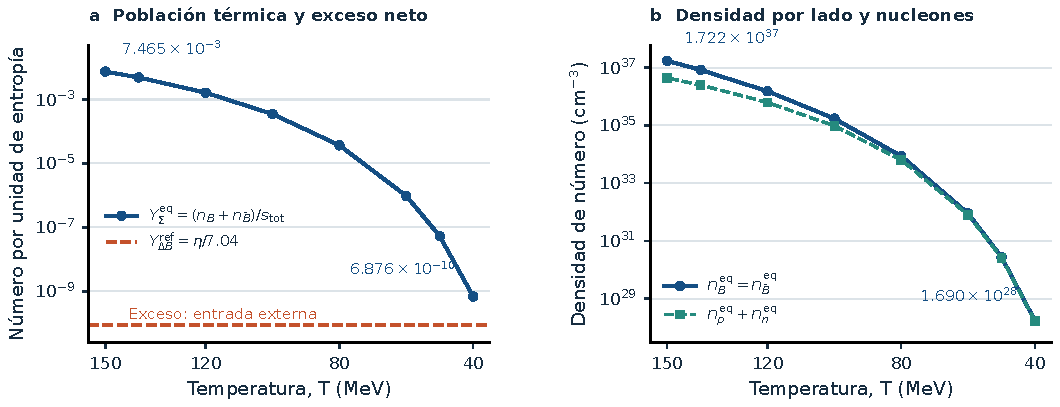
\includegraphics[width=.99\textwidth]{figures/fig04_populations_es.pdf}
\caption{Reconstrucción propia de las poblaciones numéricas con PDG2025. (a) Rendimiento térmico total $Y_\Sigma^{\rm eq}$ y exceso neto de referencia $Y_{\Delta B}^{\rm ref}=8.6932\times10^{-11}$. La línea del exceso utiliza una normalización cosmológica externa; la curva azul se calculó con el inventario HRG. (b) Densidad de cada lado simétrico y contribución de protones y neutrones. En el control simétrico, cada curva de antipartículas coincide con la de sus partículas. Los ejes siguen el enfriamiento y los segmentos guían la lectura. Son poblaciones instantáneas de equilibrio, sin contabilizar eventos acumulados de aniquilación o regeneración.}
\label{fig:populations}
\end{figure*}


\subsection{Contraste a temperatura fija}
Las tres listas ampliadas produjeron fracciones que disminuyeron en toda la malla al bajar la temperatura (Tabla~\ref{tab:comparison}; Figura~\ref{fig:comparison}). Con PDG2025 se obtuvo
\begin{align}
\fB(150\ {\rm MeV})&=0.08454533,\\
\fB(40\ {\rm MeV})&=1.7970078\times10^{-8}.
\end{align}
El primer valor equivale a 8.4545\%, mientras que el segundo equivale a $1.7970\times10^{-6}\%$.

\begin{table*}[t]\centering\footnotesize
\caption{Comparación a temperatura fija de la fracción de entropía barión-antibarión. Las cuatro columnas de $f$ son fracciones adimensionales; las dos últimas se expresan en porcentaje. La referencia reducida fue transcrita del manuscrito previo; las columnas PDG se calcularon en esta auditoría con el mismo plasma ligero. El cociente descriptivo se evaluó antes del redondeo del resultado PDG.}\label{tab:comparison}
\setlength{\tabcolsep}{9pt}\renewcommand{\arraystretch}{1.14}
\begin{tabular}{rrrrrrr}\toprule
$T$ (MeV) & $f_{\mathrm{previo}}$ & $f_{\mathrm{PDG2014}}$ & $f_{\mathrm{PDG2020}}$ & $f_{\mathrm{PDG2025}}$ & $100R$ & $100d$ \\ \midrule
150 & 0.06208 & 0.08351 & 0.08459 & 0.08455 & 73.43 & 26.57 \\
140 & 0.04328 & 0.05633 & 0.05695 & 0.05693 & 76.02 & 23.98 \\
120 & 0.01686 & 0.02018 & 0.02032 & 0.02032 & 82.97 & 17.03 \\
100 & 0.004305 & 0.004734 & 0.00475 & 0.00475 & 90.64 & 9.36 \\
80 & $5.464\times10^{-4}$ & $5.655\times10^{-4}$ & $5.661\times10^{-4}$ & $5.661\times10^{-4}$ & 96.52 & 3.48 \\
60 & $1.782\times10^{-5}$ & $1.795\times10^{-5}$ & $1.795\times10^{-5}$ & $1.795\times10^{-5}$ & 99.26 & 0.74 \\
50 & $1.148\times10^{-6}$ & $1.152\times10^{-6}$ & $1.152\times10^{-6}$ & $1.152\times10^{-6}$ & 99.67 & 0.33 \\
40 & $1.795\times10^{-8}$ & $1.797\times10^{-8}$ & $1.797\times10^{-8}$ & $1.797\times10^{-8}$ & 99.89 & 0.11 \\
\bottomrule\end{tabular}\end{table*}

\begin{figure*}[t]
\centering
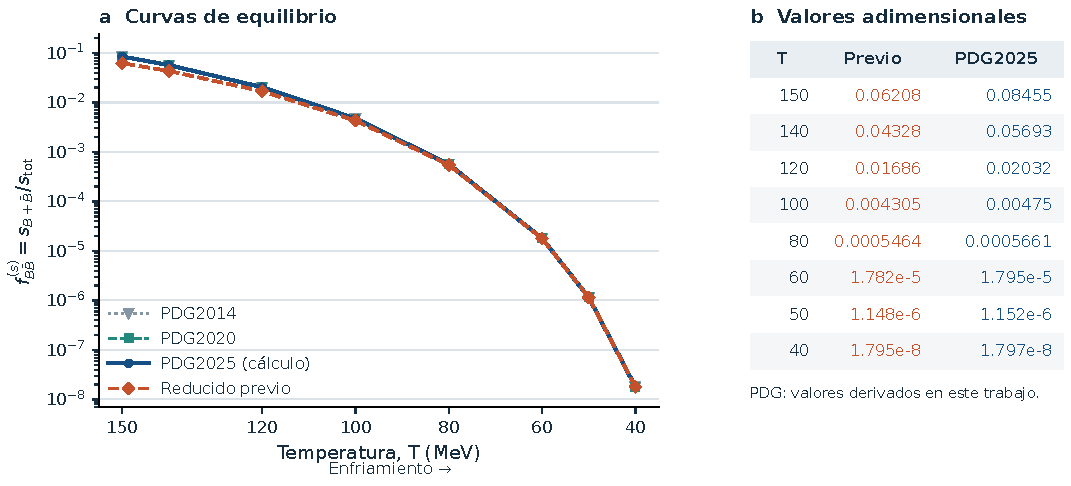
\includegraphics[width=.99\textwidth]{figures/fig01_comparison_es.pdf}
\caption{Fracción de entropía del sector barión-antibarión a potenciales químicos nulos. (a) Comparación semilogarítmica de la referencia reducida y de los tres cálculos independientes con listas de Thermal-FIST basadas en PDG2014, PDG2020 y PDG2025. El eje horizontal sigue el enfriamiento de izquierda a derecha. (b) Valores adimensionales de la referencia y del cálculo PDG2025 en las ocho temperaturas. Todas las curvas PDG son resultados derivados de este cálculo, con anchos de resonancia nulos y el mismo sector ligero en el denominador; no son mediciones externas. Los segmentos unen los puntos calculados y sirven de guía visual.}
\label{fig:comparison}
\end{figure*}

A 150 MeV, la referencia previa de 6.208\% se situó 2.2465 puntos porcentuales por debajo del cálculo PDG2025. El cociente $R$ fue 0.73428 y el déficit relativo, 26.57\%. Al enfriar, $100R$ aumentó hasta 90.64\% a 100 MeV, 99.26\% a 60 MeV y 99.89\% a 40 MeV (Figura~\ref{fig:convergence}). La variación máxima entre las tres listas en la malla se presentó a 150 MeV: 0.10775 puntos porcentuales. Sus porcentajes allí fueron 8.3509, 8.4586 y 8.4545\% para PDG2014, PDG2020 y PDG2025, respectivamente.

\begin{figure*}[t]
\centering
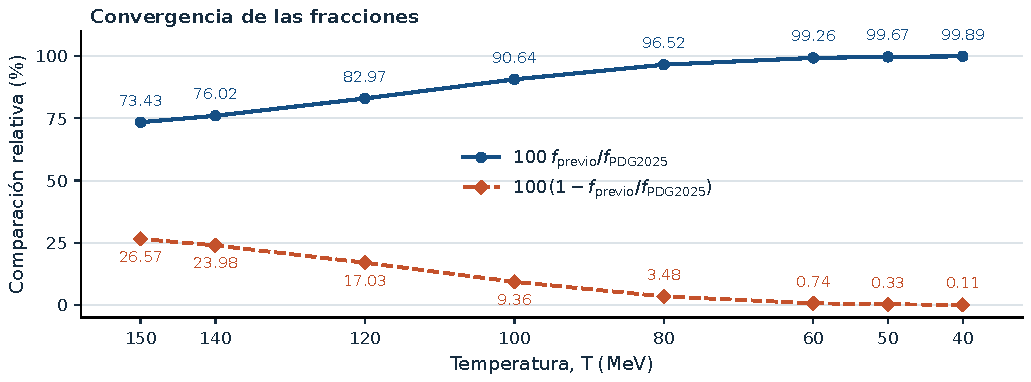
\includegraphics[width=.99\textwidth]{figures/fig02_convergence_es.pdf}
\caption{Contraste relativo entre la referencia reducida previa y el cálculo PDG2025. Los puntos azules muestran $100R=100f_{\rm previo}/f_{25}$; los naranjas, su complemento $100d=100(1-R)$. Las etiquetas contienen los valores porcentuales calculados antes del redondeo de $f_{25}$, usando los cuatro dígitos significativos disponibles para la referencia previa. Estas cantidades miden concordancia numérica entre fracciones de equilibrio; no son probabilidades de validación ni porcentajes de pares aniquilados.}
\label{fig:convergence}
\end{figure*}

\subsection{Forma de las series}
La correlación entre los logaritmos de las ocho fracciones fue $r_{\log}=0.9999233$, con $\mathrm{RMSE}_{\log}=0.0714338$. El cociente entre los extremos fue $2.89143\times10^{-7}$ para la referencia reducida y $2.12550\times10^{-7}$ para PDG2025. Las disminuciones correspondientes fueron de 6.539 y 6.673 órdenes de magnitud. La correlación de rangos de Spearman fue $\rho_S=1$, consistente con el orden monotónico compartido por ambas series. Estas métricas resumieron la forma y el contraste de amplitud de las series en la malla elegida.

\subsection{Densidades y efecto del denominador}
Con PDG2025 a 150 MeV se obtuvieron las siguientes densidades:
\begin{align}
\sB&=2.9972147\times10^{-3}\ {\rm GeV^3},\\
s_{\rm mes}&=1.1626411\times10^{-2}\ {\rm GeV^3},\\
\shad&=1.4623626\times10^{-2}\ {\rm GeV^3},\\
\sL&=2.0827352\times10^{-2}\ {\rm GeV^3},\\
\stot&=3.5450978\times10^{-2}\ {\rm GeV^3}.
\end{align}
La partición de $\stot$ fue 8.4545\% bariones y antibariones, 32.7957\% mesones y 58.7497\% sector ligero. Al utilizar sólo $\shad$ como denominador, la fracción del mismo numerador fue 20.4957\% (Figura~\ref{fig:denominator}).

\begin{figure*}[t]
\centering
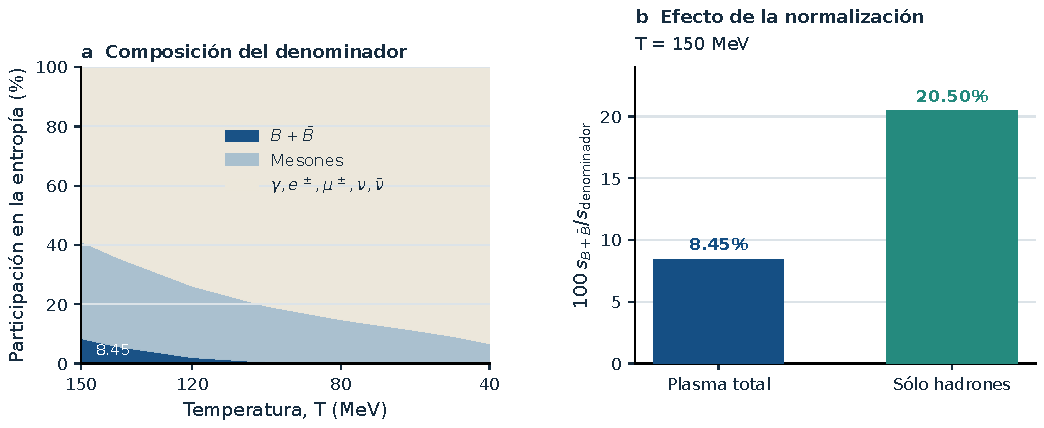
\includegraphics[width=.99\textwidth]{figures/fig03_denominator_es.pdf}
\caption{Efecto de la definición de la entropía total en el cálculo PDG2025. (a) Participación de bariones y antibariones, mesones y sector ligero en $\stot$ a las ocho temperaturas; las áreas entre puntos sólo guían la lectura. (b) El mismo numerador $\sB$ a 150 MeV representa 8.45\% de la entropía del plasma considerado y 20.50\% de la entropía exclusivamente hadrónica. El cambio se debe a la normalización, no a una población bariónica diferente. La figura representa composición instantánea de equilibrio, sin identificar el destino individual de productos de aniquilación.}
\label{fig:denominator}
\end{figure*}

\subsection{Escala del residuo y conexión con H y He}
Al normalizar por el exceso externo $\YB^{\rm ref}=8.6932\times10^{-11}$, se obtuvo $\mathcal Q(150)=8.5875\times10^7$ y $\mathcal Q(40)=7.9092$. Por cada unidad de número bariónico neto de referencia, la población simétrica inicial representó $4.2937\times10^7$ bariones y el mismo número de antibariones. Esta comparación utilizó una normalización comóvil común. A 40 MeV la población total simétrica de equilibrio aún fue 7.91 veces ese exceso; ese extremo de la malla no correspondió a un residuo final calculado.

Con las entradas observacionales y las ecuaciones~\eqref{eq:today} y \eqref{eq:hydrogen} se obtuvieron los valores de la Tabla~\ref{tab:present}. La densidad bariónica media inferida fue $(2.514\pm0.017)\times10^{-7}$ cm$^{-3}$, equivalente a $0.2514\pm0.0017$ unidades bariónicas por m$^3$. Coincidió, al redondeo de entradas, con el valor de referencia $(2.515\pm0.017)\times10^{-7}$ cm$^{-3}$ compilado por \citet{Groom2025}. Ambas conversiones compartieron la normalización del CMB.

\begin{table}[t]
\centering\small
\caption{Conversiones calculadas a partir de las entradas cosmológicas publicadas. Las incertidumbres provienen de propagación de entradas a primer orden, sin incluir errores físicos del HRG. H, He y D indican una composición primordial equivalente a la densidad media actual; no un censo de átomos neutros actuales.}
\label{tab:present}
\setlength{\tabcolsep}{3pt}\renewcommand{\arraystretch}{1.18}
\begin{tabular}{lr}\toprule
Magnitud & Densidad (${\rm cm^{-3}}$)\\\midrule
Fotones CMB & $410.73\pm0.27$\\
Número bariónico neto & $(2.514\pm0.017)\times10^{-7}$\\
Núcleos de H & $(1.898\pm0.015)\times10^{-7}$\\
Núcleos de $^4$He & $(1.540\pm0.021)\times10^{-8}$\\
Núcleos de D & $(4.760\pm0.066)\times10^{-12}$\\
\bottomrule\end{tabular}
\end{table}

La secuencia retrospectiva fue: abundancia presente, condición de conservación del exceso, propiedades del inventario HRG, temperatura elegida y solución de las poblaciones tempranas. Las conversiones H/He/D describieron la referencia cosmológica usada, sin convertirse en predicciones independientes del HRG.

\subsection{Controles numéricos y químicos}
Duplicar el número de términos de la serie no alteró las fracciones al nivel de precisión aritmética registrado. Las integrales independientes cumplieron el criterio de $10^{-8}$ para todas las especies de partícula y temperaturas verificadas. Las densidades de número verificadas mediante integrales independientes difirieron de las sumas en menos de $5\times10^{-16}$ en la precisión registrada. Se exportaron 3544 registros, correspondientes a 443 especies de partícula en ocho temperaturas. La aproximación de electrones sin masa sobreestimó su propia entropía en $1.26\times10^{-6}$ a 150 MeV y $1.77\times10^{-5}$ a 40 MeV, en términos relativos.

La solución inversa cerró la condición neta con error relativo máximo de $2.23\times10^{-15}$ en las tres listas. El cambio al duplicar los términos fue menor que $4.5\times10^{-16}$. Los excesos nucleónicos calculados mediante integrales independientes coincidieron con las sumas dentro de $3.83\times10^{-13}$ en términos relativos. A 40 MeV, incluir el exceso finito aumentó la densidad total de bariones y antibariones en 0.7961\% respecto del control simétrico. Los archivos de validación separaron esta reconstrucción de los controles a potencial nulo.
